\begin{subsection}{Operaciones de la Arquitectura}
    En este punto ya se ha formado el SDDC, la configuración de la infraestructura física y de todos los componentes de VCF está preparada para desplegar la plataforma que habilite el servicio Cloud. Este último paso se completará con los servicios que proporciona VMware con los productos que agrupa en VMware vRealize Suite, estos proporcionarán un servicio de autenticación centralizado para los usuarios y servicio de aprovisionamiento de recursos. Se utilizarán tres componentes de VMware vRealize Suite, estos son vRealize Suite Lifecycle Manager (vRSLCM), Workspace One Access (WSA) y vRealize Automation (vRA). El despliegue de estos servicios dentro del entorno será iniciado desde el componente SDDC Manager y, para aprovechar las ventajas de VMware NSX-T y las redes virtuales existentes, utilizarán como red de acceso el Segment \textit{mgmt-xRegion01-VXLAN}.

    % El entorno ya está configurado para funcionar como un SDDC, a partir de este punto ya no es necesario realizar ninguna modificación en la infraestructura física ya que todas las tareas que se deben realizar están dentro del alcance de los componentes de VMware Cloud Foundation. Para finalizar la construcción del SDDC y habilitar un servicio donde los usuarios puedan aprovisionar recursos bajo demanda, se instalarán sobre el entorno desplegado las aplicaciones Workspace ONE Access \footnote{VMware vRealize Identity Manager} (WSA) y VMware vRealize Automation (vRA). La primera permite al administrador conectar con el servidor de usuarios Active Directory y gestionarlos para proveer un servicio de autenticación centralizado a múltiples aplicaciones como VMware vRealize Automation. La segunda aplicación permite a los usuarios aprovisionar recursos de forma automatizada desde un catálogo de recursos. VMware vRealize Suite Licfecycle Manager (vRSLCM) es el componente que permite administrar vRA y WSA, su instalación y actualizaciones, las contraseñas de administrador y sus certificados, para ello necesita comunicarse con VMware vCenter Server. Se desplegará una instancia de cada componente en el \textit{management domain} creado anteriormente y estarán conectadas al \textit{segment}/subred \textit{Mgmt-xRegion01-VXLAN}.
    
    \begin{subsubsection}{vRealize Suite Lifecycle Manager}
        vRSLCM es el primer componente que se instala (este proceso se hace desde SDDC Manager) ya que es el encargado de gestionar todo lo relacionado con el resto de productos de VMware vRealize Suite.  Como su nombre indica, su función es gestionar el ciclo de vida de los servicios de VMware vRealize Suite en el SDDC, incluyendo su despliegue, actualizaciones y gestión de las credenciales de administración, certificados y licencias, por lo tanto, este componente permite al administrador controlar de forma centralizada la configuración y seguridad de los servicios dedicados a las operaciones del SDDC. Para llevar a cabo sus funciones, vRSLCM debe mantener una comunicación con la instancia de VMware vCenter Server desplegada en el Management Domain.
        % este componente está dedicado a mantener su seguridad y configuración, y a controlar que servicios se encuentran en el entorno, todo para simplificar y facilitar las tareas del administrador. Para llevar a cabo sus funciones, vRSLCM debe mantener una comunicación con la instancia de VMware vCenter Server desplegada en el Management Domain.
        \begin{figure}[h]
            \centering
            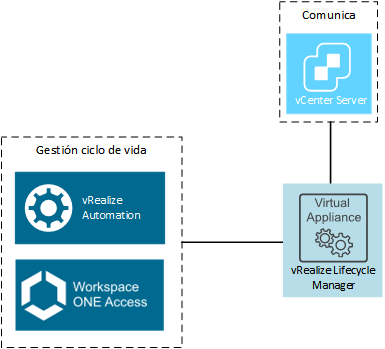
\includegraphics[width=0.4\textwidth]{imaxes/pruebaconcepto/vrealize/diseno-vrlscm.png}
            \caption{Componentes con los que se comunica vRSLCM.}
            \label{fig:vrealize-components}
        \end{figure}
        \FloatBarrier        
        Durante el despliegue de WSA y vRA, desde vRSLCM se establece su configuración, indicando la licencia, credenciales del administrador, direcciones IP, configuración DNS y NTP, y certificados para que los usuarios puedan acceder de forma segura a través del navegador\footnote{El certificado de cada aplicación es generado manualmente desde la CA y luego subido a vRSLCM, que en este caso es la VM con Windows Server 2016.}. Además, se debe elegir la ubicación donde se van a desplegar las VMs de estos servicios, es decir, el dominio de VMware vCenter Server, el cluster vSphere, la red y el datastore para el almacenamiento.
        En el entorno de pruebas, de cada servicio se crea una instancia en el Management Domain, se colocan en el cluster vSphere (\nameref{subsubsec:diseno-vsphere}), utilizan el datastore de VMware vSAN (\nameref{subsubsec:diseno-vsan}) y están controladas por la instancia de VMware vCenter Server (\nameref{subsubsec:diseno-vcenter}). Como ya se ha mencionado, las instancias se conectan a un Segment controlado por VMware NSX-T (como se muestra en la figura \ref{fig:two-tier-topology}) para poder hacer uso de sus servicios de red.
        \begin{figure}[h]
            \centering
            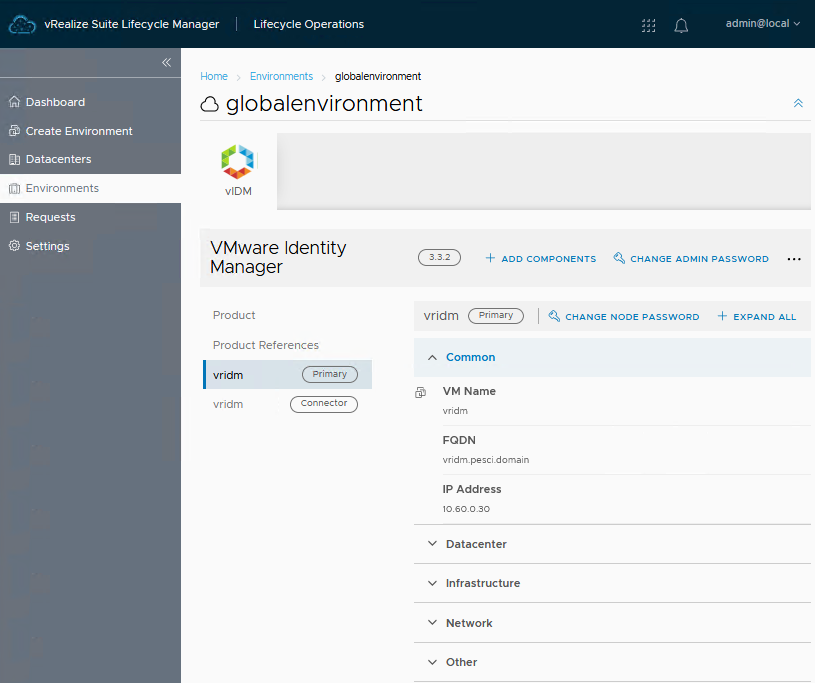
\includegraphics[width=0.6\textwidth]{imaxes/pruebaconcepto/vrealize/config-istance-vridm.png}
            \caption{Apartado donde se muestra la configuración de la instancia de WSA en vRSLCM.}
            \label{fig:config-WSA}
        \end{figure}
        \FloatBarrier 
        
        % Dentro de vRSLCM, los despliegues son organizados por entornos pudiendo crearse un entorno por cada servicio o un entorno con todos los servicios. Existen dos modos de despliegue, uno donde se crean tres instancias del servicio para balancear la carga\footnote{El balanceo de la carga se realiza con el servicio de Load Balancing de VMware NSX-T.}, y otro donde solo se crea una instancia.

        % En el entorno, se despliega una instancia de cada servicio. Estas están colocadas bajo el dominio de la instancia de VMware vCenter en el cluster vSphere

        % Este se instala desde SDDC Manager, pero una vez instalado es utilizado para desplegar cualquier servicio de VMware vRealize Suite.
        
    \end{subsubsection}

    \begin{subsubsection}{Workspace One Access}
        WSA es el componente de VMware vRealize Suite que se integra con un directorio de usuarios para proporcionarles acceso a las aplicaciones que se despliegan en el entorno, vRA en este caso. Así, en el entorno de producción, WSA se utilizaría para que los usuarios del SDDC se pudieran conectar utilizando sus credenciales de la UDC, ya que estaría conectado al directorio de la universidad.        
        En el entorno de pruebas, se integra con el directorio de usuarios Active Directory situado en la VM con Windows Server 2016. Este Active Directory contiene perfiles de usuarios y grupos de usuarios organizados en unidades organizativas, los perfiles de usuario se añaden a grupos de usuarios, y la creación y mantenimiento de sus credenciales se realiza desde el propio Active Directory. Desde WSA se seleccionan los usuarios y grupos de usuarios que se quieran sincronizar para que estén disponibles en el SDDC y, posteriormente, desde cada aplicación se determina el nivel de acceso y permisos para cada usuario. Como norma general se deben asignar permisos a grupos de usuarios y no a perfiles individuales, de esta forma se reduce el tiempo de gestión y se simplifica la estructura, ya que para asignar nuevos permisos a un usuario solo sería necesario añadirlo al grupo correspondiente.        
        En Active Directory se han configurado varios usuarios que se sincronizan en WSA. Estos se utilizarán para mostrar las funcionalidades de vRA como si se tratase del entorno de producción con perfiles de usuarios de la UDC.
        \begin{figure}[h]
            \centering
            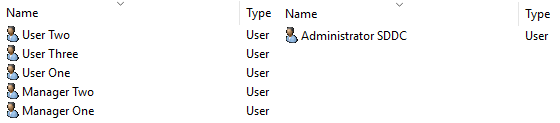
\includegraphics[width=0.6\textwidth]{imaxes/pruebaconcepto/vrealize/users-AD.png}
            \caption{Usuarios dentro de Active Directory}
            \label{fig:users-defined-AD}
        \end{figure}        
        Desde WSA se seleccionan aquellas unidades organizativas que se quieren sincronizar. Cada unidad contiene usuarios y grupos de usuarios, los usuarios que harán uso del servicio de aprovisionamiento están colocados en la unidad CITIC. 
        \begin{figure}[h]
            \centering
            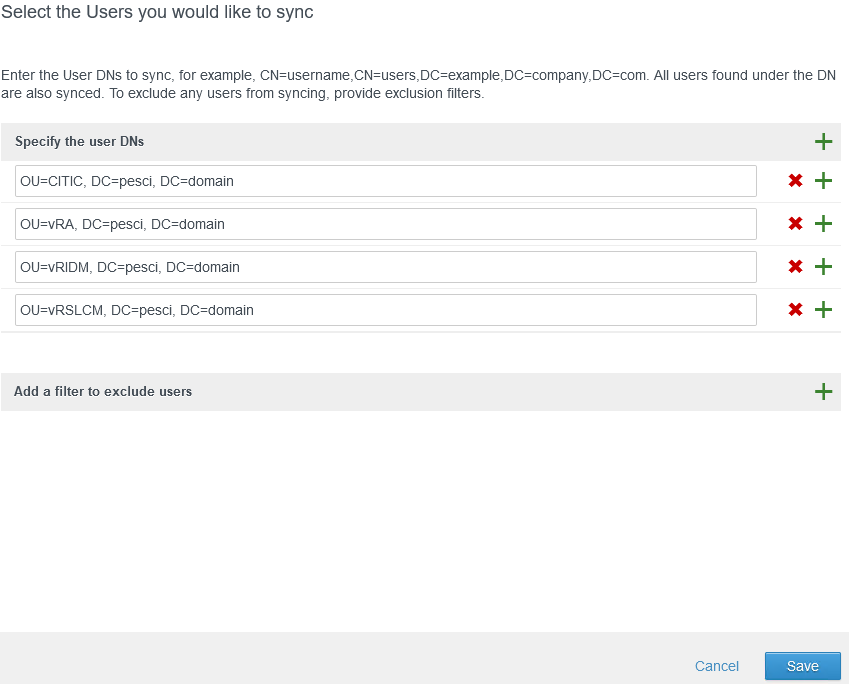
\includegraphics[width=0.6\textwidth]{imaxes/pruebaconcepto/vrealize/syncing-users.png}
            \caption{Sincronización de usuarios desde Workspace One Access.}
            \label{fig:users-defined-WSA}
        \end{figure}
        \FloatBarrier
        \begin{figure}[h]
            \centering
            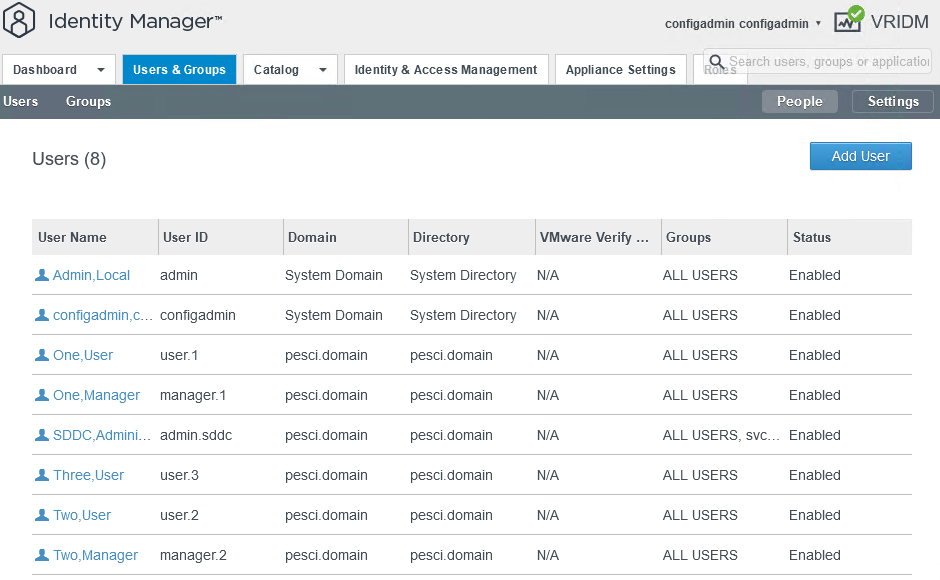
\includegraphics[width=0.6\textwidth]{imaxes/pruebaconcepto/vrealize/users-wsa.png}
            \caption{Usuarios sincronizados en Workspace One Access.}
            \label{fig:users-defined-WSA}
        \end{figure}
        \FloatBarrier
        El acceso a las aplicaciones está centralizado a través de una plataforma proporcionada por WSA. Cuando el usuario intenta acceder a vRA este es redirigido a una página web donde introduce sus credenciales, WSA comprueba los datos introducidos y vuelve a redirigir al usuario a la plataforma de vRA. Además, utilizando esta plataforma el administrador puede obtener estadísticas sobre que usuarios se autentican, a que servicios acceden y desde donde lo hacen. WSA permite al administrador editar la interfaz de la web de autenticación, pudiendo personalizar el icono y nombres que se muestran, y modificar los parámetros que se utilizan para autenticarse o mantener las sesiones, permitiendo definir si el usuario debe utilizar su cuenta de correo electrónico o nombre de usuario y si se utilizan cookies de sesión o persistentes. Por si esto fuera poco, también existe la posibilidad de crear políticas para controlar como se autentican los usuarios, desde donde pueden hacerlo y el tiempo de duración de la sesión. En la siguiente figura se muestran las reglas de la política por defecto que se aplica a los usuarios, se permite el acceso desde cualquier dirección IP, a través de un navegador web o la aplicación para dispositivos móviles Workspace One App, usando su contraseña y con un tiempo de sesión de 2160 u 8 horas dependiendo del punto de acceso.
        \begin{figure}[h]
            \centering
            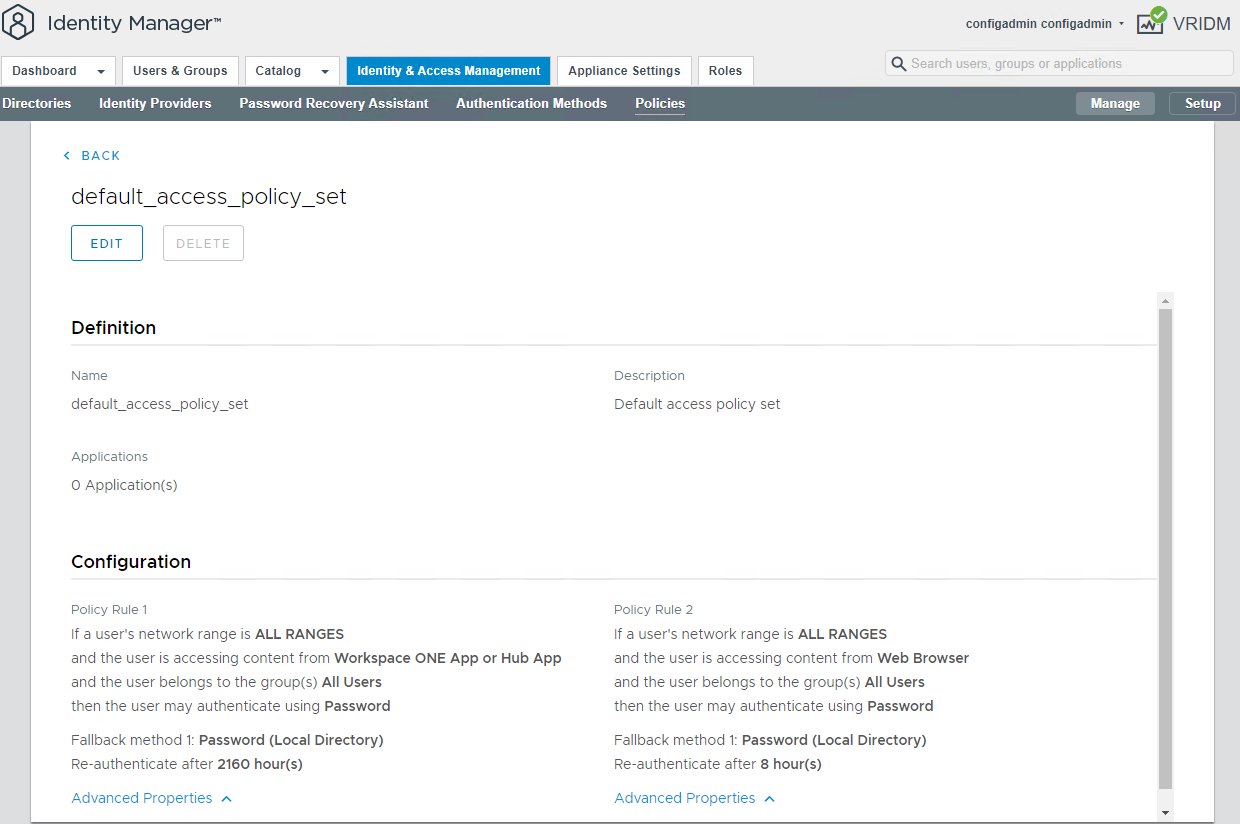
\includegraphics[width=0.6\textwidth]{imaxes/pruebaconcepto/vrealize/default-policy.png}
            \caption{Política de autenticación por defecto.}
            \label{fig:default-policy}
        \end{figure}
        \FloatBarrier
        
        \begin{figure}[h]
            \centering
            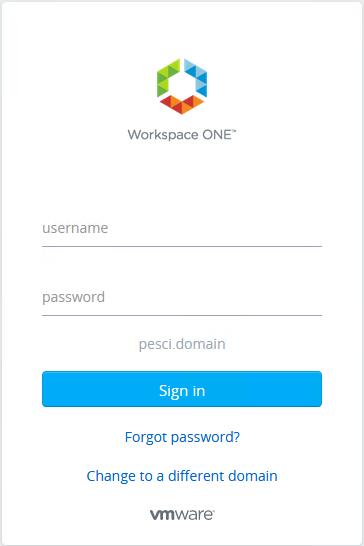
\includegraphics[width=0.3\textwidth]{imaxes/pruebaconcepto/vrealize/wsa-login.png}
            \caption{Plataforma de autenticación de Workspace One Access}
            \label{fig:wsa-platform}
        \end{figure}
        \FloatBarrier        
        Con WSA el administrador tiene un mayor control sobre los usuarios y como estos acceden a los servicios de la plataforma Cloud, ya que gestiona desde un único punto todas las cuentas de usuarios y la seguridad del punto de acceso, pudiendo controlar que usuarios acceden y estableciendo medidas seguridad de forma sencilla e intuitiva. También, la gestión de las credenciales de cada usuario se separa de la gestión del acceso, ya que lo primero está controlado por Active Directory y lo segundo por WSA. De esta forma, la seguridad del entorno aumenta y las tareas del administrador se simplifican. Con esta plataforma se soluciona uno de los problemas de la infraestructura del CITIC, ya no es necesario crear cuentas manualmente para cada usuario que quiera acceder al servicio y su gestión se hace más dinámica, a la vez que se aumenta el nivel de seguridad.

        % Los usuarios que necesiten acceder a vRA deben estar registrados en el directorio de Workspace One Access. Este componente centraliza el acceso de todos los productos de VMware vRealize. Cuando se despliega se debe configurar un Active Directory que en el caso del entorno está situado en la VM con Windows Server 2016. Dentro del Active Directory existen grupos de seguridad y perfiles de usuario, un perfil de usuario contiene información como nombre, apellidos, dirección e-mail, nombre de usuario y contraseña\footnote{Se pueden configurar más campos pero los que se describen son los obligatorios a la hora de crear un usuario.}, y este puede formar parte de varios grupos de seguridad. Una vez configurado, cada aplicación se conectará a WSA y se podrán asignar roles para los grupos de seguridad y usuarios estableciendo así un nivel de acceso. Además, cada usuario registrado tendrá disponible un catálogo de aplicaciones en el portal de WSA cuyo administrador establecerá que aplicaciones están habilitadas para cada usuario o grupo, eso sí, para que el usuario pueda acceder a ella previamente se debe establecer un rol para ese usuario dentro de la aplicación.

        %*****USUARIOS QUE HAY EN EL ENTORNO Y EL ACCESO A CADA APLICACIÓN*******%
        % \begin{figure}[h]
        %     \centering
        %     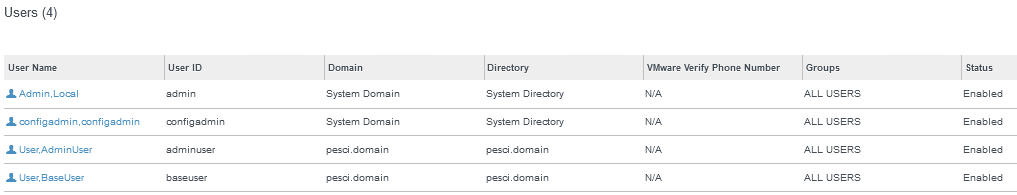
\includegraphics[width=0.4\textwidth]{imaxes/vRealize_pruebaconcepto/usuariosDefinidos.png}
        %     \caption{Muestra los usuarios definidos en el Active Directory sincronizados en Workspace One Access.}
        %     \label{fig:users-defined-AD}
        % \end{figure}
        % \FloatBarrier
        % En la Figura \ref{fig:users-defined-AD} se muestran los dos usuarios definidos en el Active Directory y dos usuarios que se corresponden a los perfiles de administración de WSA, no se utilizarán grupos de seguridad para reducir la complejidad pero su configuración en las aplicaciones de VMware es igual que para los perfiles de usuario. En un entorno real existen usuarios que controlan a otros usuarios y establecen su nivel de acceso, a parte de los perfiles de administrador de cada aplicación. Para el entorno se define el perfil \textit{adminuser} que será el encargado de gestionar el acceso de dos usuarios (\textit{baseuser1} y \textit{baseuser2}) que serán los que consuman a las aplicaciones desplegadas (vRSLCM y vRA). El primero tendrá acceso y permisos de edición en las aplicaciones vRSLCM y vRA, mientras que los dos usuarios base solo podrán acceder a vRA y dentro de este el usuario admin definirá que servicios están habilitados para cada uno.

        %************************************************************************%

    \end{subsubsection}

    \begin{subsubsection}{VMware vRealize Automation}
        VMware vRealize Automation es el componente de VMware vRealize Suite que automatiza el aprovisionamiento de recursos del SDDC. Con esta plataforma los usuarios podrán elaborar diseños de los recursos que necesitan para posteriormente implementarlos y llevar a cabo sus trabajos. El proceso de implementación es automático y transparente para el usuario que puede modificar los requisitos de sus recursos según sea necesario. Al mismo tiempo, el administrador establece los límites de las diseño/implementación y debe proveer los medios que se usarán como base para los diseños.
        


        El punto a través del cual los usuarios pueden aprovisionar sus recursos es vRealize Automation. Este producto provee el servicio cloud. 
        \begin{figure}[h]
            \centering
            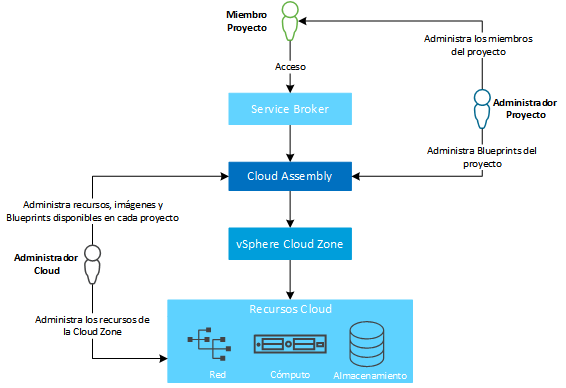
\includegraphics[width=0.8\textwidth]{imaxes/vRealize_pruebaconcepto/ComponentesVRA.png}
            \caption{Componentes de VMware vRealize Automation y tareas que realiza cada rol de usuario.}
            \label{fig:vra-components}
        \end{figure}
        \FloatBarrier
        Internamente vRA se divide en varios servicios que permiten gestionar los diferentes aspectos de la cloud. Para centrarse en los objetivos de este proyecto solo se hace referencia a dos de esos servicios, el primero es Cloud Assembly el cual permite administrar la infraestructura disponible controlar el uso que se hace de esos recursos, y el segundo es Service Broker, utilizado por los usuarios para aprovisionar los recursos desde un catálogo de plantillas. La obtención de los recursos por parte del usuario se hace desplegando una serie de plantillas llamadas Blueprints diseñadas previamente, en donde se define un conjunto de VMs y recursos de red y de almacenamiento incluyendo otros aspectos como la configuración de cada uno de los recursos, como redes de la infraestructura que se utilizan, cantidad de almacenamiento, o la ubicación del despliegue en la infraestructura. Son ficheros de código con extensión \textit{.yaml} donde se indican etiquetas, aunque también se pueden diseñar con un editor gráfico. Estas plantillas están relacionadas con proyectos, una plantilla pertenece a uno o varios proyectos donde existe un coordinador de proyecto que se encarga de diseñar Blueprints y de administrar los usuarios miembros de ese proyecto. Los proyectos de vRA permiten limitar los recursos para que un conjunto de usuarios pueda desplegar los componentes definidos en las Blueprints disponibles, como la cantidad de memoria RAM, cantidad de instancias que se pueden desplegar y cantidad de almacenamiento, también aquellas redes que se pueden utilizar. Desde el punto de vista de vRA, la infraestructura se divide en Cloud Zones, las cuales son conjuntos de recursos situados en distintos proveedores Cloud que pueden ser públicos como AWS o Azure, o privados que solo pueden ser clusters vSphere. En el caso del entorno desplegado solo se tendrá una única Cloud Zone de tipo vSphere. En cada Cloud Zone se define como se deben distribuir los recursos aprovisionados sobre la infraestructura. 
        Finalmente será el administrador de la infraestructura el que se encargue de proveer los recursos, administrar los proyectos disponibles, gestionar los coordinadores de cada proyecto y controlar y limitar el uso de los recursos.
        % Finalmente, vRA permite configurar tarjetas donde se puede definir el coste del aprovisionamiento de CPU, almacenamiento y memoria RAM, además del coste de uso de otros elementos como sistemas operativos, el uso de una determinada red o el uso de una determinada Cloud Zone. Estas tarjetas se asignan por proyecto para determinar el coste que tendrá el consumo de recursos por mes.


    \end{subsubsection}

    
\end{subsection}